\chapter{Reproducción y detalles de los modelos}
\label{ap:general}
\addtocontents{toc}{\protect\setcounter{tocdepth}{0}}

\section{Reproducción}
\label{ap:reproduccion}

El código corre en macOS 13 o posterior, o en Linux, con 8\,GB de RAM y sin GPU. El archivo \texttt{entorno.yml} fija las versiones de Python 3.13, scikit-learn 1.9.1 \citep{pedregosa2011}, LightGBM 4.7.0, XGBoost 3.4.2, CatBoost 1.2.10, statsforecast 2.1.1 y las demás librerías, y todas las semillas son fijas.

\begin{lstlisting}[language=bash]
cd tesis-sipsa       # carpeta del repositorio
bash preparar.sh     # una vez: crea el entorno con entorno.yml
bash correr.sh       # corre todos los pasos y genera tablas y figuras
\end{lstlisting}

Las entradas son dos archivos de la carpeta \texttt{datos}: la base mensual del SIPSA (\texttt{base\_unida\_mensual.parquet}) y la serie del ONI (\texttt{oni\_v6.csv}). La base mensual la construyó el autor con los programas de la carpeta \texttt{preparacion\_datos}, a partir de los archivos de abastecimiento (SIPSA-A) y de precios mayoristas (SIPSA-P) publicados por el DANE \citep{dane}: se unifican los archivos semestrales y los anexos mensuales, se suman las toneladas por central, producto y mes, y se cruzan con los precios por nombre del producto, con las equivalencias de variedades descritas en la sección~\ref{sec:carga}. La elección de la variedad de referencia con datos hasta diciembre de 2024 se aplica con el programa \texttt{corregir\_variedad.py}, que deja un informe de los pares modificados. Los archivos originales del DANE y la serie del ONI se descargaron a comienzos de noviembre de 2026 de las páginas citadas en la bibliografía; los archivos de entrada usados tienen estas sumas SHA-256, guardadas en \texttt{datos/SHA256SUMS.txt}:

\begin{lstlisting}
f8117feee753bf7c8df16d5defdd6cae146c57540cf24c7ae393afce82b35fb6  base_unida_mensual.parquet
2b1c5b6a28cd11f145790589570dec364cc7cb3fd9f30f8cc9254f00d0cfceb5  oni_v6.csv
\end{lstlisting}

El código, los datos de entrada, los modelos guardados y este documento en LaTeX están en el repositorio público \url{https://github.com/misebastian/tesis-sipsa}; su archivo \texttt{README.md} indica cómo instalar el entorno y repetir la corrida. Los archivos originales del DANE no se incluyen por su tamaño y se descargan de las páginas citadas. El repositorio contiene también una página web, \url{https://tesis-sipsa.vercel.app}, que muestra para cada alimento y central el pronóstico del mes siguiente, su rango y la alerta de alza fuerte calculados con el modelo final; un programa construye las variables del último mes publicado con el mismo código del panel y aplica los modelos guardados. Cada paso guarda sus resultados en la carpeta \texttt{resultados}; al final, un programa produce las figuras y otros las tablas y cifras de este documento. Los pasos 4, 5 y 12 guardan los modelos finales en \texttt{resultados/modelos}, de modo que las explicaciones se calculan sobre el mismo objeto que se evalúa. Todos los resultados provienen de una sola corrida completa en el computador descrito en la tabla~\ref{tab:tiempos}, que muestra el tiempo y la memoria de cada paso; la única excepción es el AUC de la validación adversaria con solo el cambio del mes siguiente, que se calculó con el mismo código y el mismo panel en un servidor Linux con las mismas versiones de las librerías.

\begin{table}[htbp]\centering\footnotesize
\caption{Tiempo de ejecución y memoria residente máxima por programa, medidos con \texttt{medir.py} en la corrida de referencia (Darwin arm64, 10 núcleos)}\label{tab:tiempos}
\begin{adjustbox}{max width=\textwidth}\begin{tabular}{lp{6.4cm}rr}\toprule
Programa & Qué hace & Minutos & Memoria (GB)\\ \midrule
\texttt{01\_panel.py} & Panel supervisado y variables candidatas & 0{,}1 & 0{,}83 \\
\texttt{02\_eda.py} & Análisis exploratorio y calidad & 0{,}2 & 0{,}77 \\
\texttt{03\_variables.py} & Selección de variables (validación) & 8{,}2 & 0{,}69 \\
\texttt{sarima.py} & SARIMA por serie (todos los cortes) & 19{,}7 & 0{,}47 \\
\texttt{04\_regresion.py} & Búsqueda y prueba de los modelos de regresión & 14{,}1 & 0{,}98 \\
\texttt{05\_clasificacion.py} & Búsqueda, balanceo, recalibración, umbral y prueba de los clasificadores & 27{,}9 & 0{,}81 \\
\texttt{06\_resultados.py} & Métricas, bootstrap, pruebas, figuras e importancia & 18{,}1 & 0{,}64 \\
\texttt{07\_complementarios.py} & Origen móvil, cuantiles, CQR y faltantes & 18{,}3 & 1{,}13 \\
\texttt{09\_verificacion.py} & Verificación de implementaciones & 0{,}1 & 1{,}39 \\
\midrule Total & & 107 & 1{,}39 \\
\bottomrule\end{tabular}\end{adjustbox}\end{table}


\begin{table}[htbp]\centering\small
\caption{Costo computacional. Complejidad aproximada de un ajuste ($n$ observaciones, $p$ variables) y tiempo medido de la búsqueda de hiperparámetros en segundos (40 configuraciones $\times$ 3 cortes = 120 ajustes, salvo las que se ampliaron según la tabla~\ref{tab:hiper}, en paralelo con 10 núcleos).}\label{tab:costo}
\begin{adjustbox}{max width=\textwidth}\begin{tabular}{llp{4.3cm}rr}\toprule
& & & \multicolumn{2}{c}{Tiempo de búsqueda (s)}\\ \cmidrule(lr){4-5}
Modelo & Complejidad & Parámetros & Regresión & Clasificación\\ \midrule
Regresión cuantílica / logística & $O(E\,n\,p)$ & pasadas $E$ sobre los datos & 17 & 92 \\
MLP & $O(E\,n\,p\,h)$ & $h$ neuronas por capa & 165 & 101 \\
Random Forest & reg.: $O(B\,n\,p)$; clas.: $O(B\,m\,n\log n)$ & reg.: bosque de LightGBM con histogramas; clas.: scikit-learn, $m$ variables por división & 150 & 1009 \\
XGBoost & $O(M\,n\,p)$ & $M$ árboles, cortes por histogramas & 119 & 55 \\
LightGBM & $O(M\,n\,p)$ & $M$ árboles, cortes por histogramas & 74 & 74 \\
CatBoost & $O(M\,n\,p)$ & $M$ árboles simétricos & 130 & 191 \\
\bottomrule\end{tabular}\end{adjustbox}\end{table}


\section{Definición de las variables candidatas}
\label{ap:variables}

\footnotesize
\begin{longtable}{>{\raggedright\arraybackslash}p{2.3cm}>{\raggedright\arraybackslash}p{4.1cm}>{\raggedright\arraybackslash}p{6.2cm}c}
\caption{Definición de las 52 variables candidatas. Notación: $l_t=\ln p_t$ con el último precio repetido en huecos de hasta dos meses; $r_t=l_t-l_{t-1}$; $a_t=1\{r_t>\ln 1{,}15\}$; $o_t$, promedio de $l_t$ en las demás centrales que cotizan el producto; $T_t$, logaritmo de las toneladas; $m_{t+1}$, mes del año pronosticado. Las ventanas móviles exigen al menos tres cuartas partes de los meses. Final: variable incluida en los modelos.}\label{tab:variables}\\
\toprule Bloque & Variable & Definición & Final\\ \midrule\endfirsthead
\toprule Bloque & Variable & Definición & Final\\ \midrule\endhead
\bottomrule\endfoot
Historia del precio & Cambio del precio, 1 mes & $l_t-l_{t-1}$ & Sí \\
 & Cambio del precio, 2 meses & $l_t-l_{t-2}$ & Sí \\
 & Cambio del precio, 3 meses & $l_t-l_{t-3}$ & Sí \\
 & Cambio del precio, 6 meses & $l_t-l_{t-6}$ & Sí \\
 & Cambio del precio, 12 meses & $l_t-l_{t-12}$ & Sí \\
 & Cambio mensual hace 1 mes & $r_{t-1}$ & Sí \\
 & Cambio mensual hace 2 meses & $r_{t-2}$ & Sí \\
 & Cambio mensual hace 3 meses & $r_{t-3}$ & Sí \\
 & Volatilidad 3 meses & desv. típica de $r$ en $t-2,\dots,t$ & Sí \\
 & Volatilidad 6 meses & desv. típica de $r$ en $t-5,\dots,t$ & No \\
 & Volatilidad 12 meses & desv. típica de $r$ en $t-11,\dots,t$ & Sí \\
 & Posición del precio en el año (z) & $(l_t-\bar l_{12})/s_{12}$, media y desv. de $l$ en 12 meses & Sí \\
 & Distancia al máximo anual & $l_t-\max_{12}l$ & Sí \\
 & Distancia al mínimo anual & $l_t-\min_{12}l$ & Sí \\
 & Alzas fuertes en el último año & $\sum_{k=0}^{11}a_{t-k}$ & No \\
 & Meses desde la última alza & meses desde el último $a=1$ (tope 24) & Sí \\
\addlinespace[2pt]
Estacionalidad & Mes del año (seno) & $\sin(2\pi m_{t+1}/12)$ & Sí \\
 & Mes del año (coseno) & $\cos(2\pi m_{t+1}/12)$ & Sí \\
 & Frecuencia histórica de alzas en el mes & $(k+1)/(n+6)$: alzas $k$ del producto en el mes $m_{t+1}$ en $n$ registros de años anteriores & Sí \\
 & Cambio histórico en el mes & media de $r$ de la serie en el mes $m_{t+1}$ en años anteriores & Sí \\
\addlinespace[2pt]
Abastecimiento local & Cambio de toneladas, 1 mes & $T_t-T_{t-1}$ & No \\
 & Cambio de toneladas, 12 meses & $T_t-T_{t-12}$ & No \\
 & Toneladas frente a su promedio anual & $T_t-$ media de $T$ en $t-12,\dots,t-1$ & No \\
 & Municipios de origen (log) & $\ln(1+$municipios de origen$)$ & No \\
 & Departamentos de origen & departamentos de origen & No \\
 & Días con registro & días con registro de toneladas & No \\
\addlinespace[2pt]
Red de centrales & Brecha con las demás centrales & $l_t-o_t$ & Sí \\
 & Cambio en las demás centrales, 1 mes & $o_t-o_{t-1}$ & Sí \\
 & Demás centrales con alza en t & proporción de las demás centrales con $a_t=1$ & Sí \\
\addlinespace[2pt]
Calendario & Semana Santa & 1 si Semana Santa cae en $t+1$ & No \\
 & Diciembre & 1 si $t+1$ es diciembre & No \\
\addlinespace[2pt]
Producto y lugar & Perecibilidad & 0 granos y procesados; 1 tubérculos, lácteos y pescados; 2 frutas y verduras & Sí \\
 & Grupo (código) & código entero del grupo & Sí \\
 & Ciudad (código) & código entero de la ciudad & Sí \\
 & Central (código) & código entero de la central & Sí \\
 & Producto (código) & código entero del producto & Sí \\
\addlinespace[2pt]
El Niño (ONI) & ONI & ONI de $t-2$ & No \\
 & Cambio del ONI, 3 meses & ONI$_{t-2}-$ONI$_{t-5}$ & No \\
\addlinespace[2pt]
Promedios móviles & Desviación de la media móvil 3m & $l_t-$ media de $l$ en 3 meses & No \\
 & Desviación de la media móvil 6m & $l_t-$ media de $l$ en 6 meses & No \\
\addlinespace[2pt]
Año anterior & Cambio del mismo mes, año anterior & $r_{t-10}$ (cambio del mes objetivo un año antes) & No \\
 & Cambio en las demás centrales, mismo mes del año anterior & $o_{t-10}-o_{t-11}$ & No \\
\addlinespace[2pt]
Red ampliada & Cambio en las demás centrales, 2 meses & $o_t-o_{t-2}$ & No \\
 & Cambio en las demás centrales, 12 meses & $o_t-o_{t-12}$ & No \\
 & Cambio de la brecha con las demás centrales & $(l_t-o_t)-(l_{t-1}-o_{t-1})$ & No \\
\addlinespace[2pt]
Grupo en la central & Cambio del grupo en la central & media de $r_t$ de los demás productos del grupo en la central & No \\
 & Alzas del grupo en la central & proporción de $a_t=1$ en los demás productos del grupo en la central & No \\
\addlinespace[2pt]
Abastecimiento nacional & Cambio de toneladas en todas las centrales & cambio de $\ln$ toneladas del producto en todas las centrales & Sí \\
 & Toneladas en todas las centrales frente al año & $\ln$ toneladas en todas las centrales frente a su media de 12 meses & Sí \\
 & Participación de la central en las toneladas & toneladas de la central / toneladas en todas las centrales & Sí \\
\addlinespace[2pt]
Calidad del dato & Meses con precio en el año & meses con precio observado en $t-11,\dots,t$ & No \\
 & Días con registro frente al año & días con registro frente a su media de 12 meses & No \\
\end{longtable}
\normalsize


\section{Detalles de los modelos}
\label{ap:modelos}



\subsection*{Hiperparámetros}

Los espacios de búsqueda están en la tabla~\ref{tab:espacios}. La tabla~\ref{tab:hiper} muestra los valores elegidos para cada modelo. Las búsquedas de regresión y de clasificación usaron la misma semilla y, por tanto, la misma secuencia de configuraciones; en Random Forest, la configuración 20 fue la mejor en ambas tareas, por lo que sus hiperparámetros coinciden. Se verificó en los archivos de la búsqueda que no se trata de un error de transcripción. La figura~\ref{fig:busqueda} muestra el mejor resultado de validación según el número de configuraciones evaluadas. Todas las búsquedas se detuvieron con las 40 configuraciones iniciales, salvo la de XGBoost en regresión: su mejor configuración fue la 39, de modo que la mejora en las últimas diez superó la tolerancia y la búsqueda se amplió a 60 configuraciones, sin nuevas mejoras.

\begin{figure}[htbp]\centering
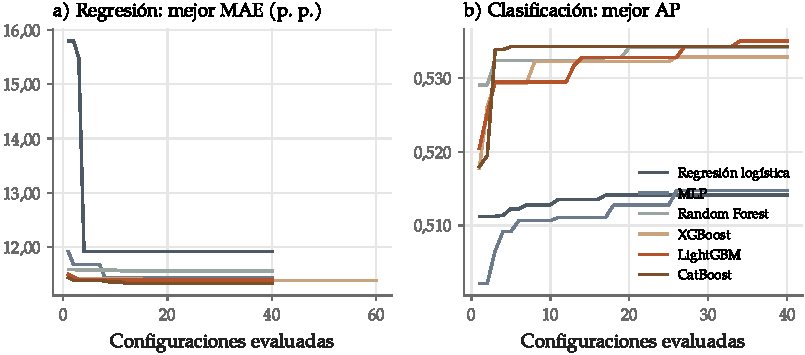
\includegraphics[width=.8\textwidth]{fig_busqueda}
\caption{Convergencia de la búsqueda aleatoria: mejor MAE promedio de validación (a) y mejor AP de validación (b) según el número de configuraciones evaluadas.}\label{fig:busqueda}
\end{figure}
\FloatBarrier

\footnotesize
\begin{longtable}{llrp{7.4cm}}
\caption{Hiperparámetros elegidos por búsqueda aleatoria (número de configuraciones evaluadas en la tercera columna). Las dos búsquedas de cada modelo usaron la misma semilla y, por tanto, la misma secuencia de configuraciones; en Random Forest, la misma configuración resultó la mejor en ambas tareas, por lo que sus valores coinciden.}\label{tab:hiper}\\
\toprule Tarea & Modelo & $N$ & Valores elegidos\\ \midrule\endfirsthead
\toprule Tarea & Modelo & $N$ & Valores elegidos\\ \midrule\endhead
\bottomrule\endfoot
Reg. & Regresión cuantílica & 40 & $\alpha$ $3{,}4\cdot10^{-7}$; penal. L1 \\
Reg. & MLP & 40 & $\alpha$ 0{,}0067; capas (128, 64); tasa 0{,}0019 \\
Reg. & Random Forest & 40 & hoja mín. 21; frac. var. 0{,}405; prof. 19 \\
Reg. & XGBoost & 60 & frac. col. 0{,}451; tasa 0{,}022; peso mín. 7{,}370; árboles 424; prof. 7; submuestra 0{,}751 \\
Reg. & LightGBM & 40 & frac. col. 0{,}636; hojas 33; $\lambda$ 0{,}0019; tasa 0{,}023; obs. hoja 135; árboles 581; submuestra 0{,}948 \\
Reg. & CatBoost & 40 & $\lambda$ 2{,}288; tasa 0{,}044; árboles 307; prof. 7 \\
\midrule
Clas. & Regresión logística & 40 & $C$ 0{,}0030; penal. L1 \\
Clas. & MLP & 40 & $\alpha$ $1{,}9\cdot10^{-5}$; capas (64); tasa $2{,}0\cdot10^{-4}$ \\
Clas. & Random Forest & 40 & hoja mín. 21; frac. var. 0{,}405; prof. 19 \\
Clas. & XGBoost & 40 & frac. col. 0{,}573; tasa 0{,}040; peso mín. 21{,}485; árboles 190; prof. 6; submuestra 0{,}637 \\
Clas. & LightGBM & 40 & frac. col. 0{,}722; hojas 89; $\lambda$ 9{,}149; tasa 0{,}029; obs. hoja 83; árboles 166; submuestra 0{,}705 \\
Clas. & CatBoost & 40 & $\lambda$ 4{,}448; tasa 0{,}039; árboles 447; prof. 4 \\
Cuant. & LightGBM & 40 & frac. col. 0{,}808; hojas 12; $\lambda$ 8{,}209; tasa 0{,}025; obs. hoja 106; árboles 611; submuestra 0{,}765 \\
\end{longtable}
\normalsize


\clearpage
\subsection*{Verificación de las implementaciones propias}

La regresión cuantílica por descenso de gradiente se comparó con la solución exacta en una submuestra; la red neuronal con pérdida absoluta, comparando su gradiente con diferencias finitas y comprobando en datos simulados que estima la mediana y no la media, y el Random Forest de LightGBM, con el de scikit-learn con los mismos hiperparámetros. Las tres coinciden con su referencia (tabla~\ref{tab:verificacion}). En la regresión cuantílica, la correlación entre los coeficientes (0,77) es menor que entre las predicciones (0,998), porque varias variables están muy correlacionadas entre sí y distintas combinaciones de coeficientes dan casi el mismo ajuste. El bosque de LightGBM tiene un error 0,19 puntos mayor que el de scikit-learn en la submuestra, con predicciones muy correlacionadas.

\begin{table}[htbp]\centering\footnotesize
\caption{Verificación de las implementaciones no estándar (submuestras de 6\,000 y 3\,000 filas de entrenamiento, 4\,000 de validación; simulación con ruido exponencial centrado en la mediana)}\label{tab:verificacion}
\begin{adjustbox}{max width=\textwidth}\begin{tabular}{llr}\toprule
Implementación & Comprobación & Resultado\\ \midrule
Regresión cuantílica & MAE (p.\,p.) solución exacta / descenso de gradiente & 11{,}58 / 11{,}59 \\
 & Correlación de predicciones / de coeficientes & 0{,}9979 / 0{,}769 \\
MLP (error absoluto) & Error relativo del gradiente, mediana / máximo & $1{,}8\cdot10^{-9}$ / $8{,}1\cdot10^{-6}$ \\
 & Simulación: distancia a la mediana / a la media (pérdida absoluta) & 0{,}059 / 0{,}334 \\
 & Simulación: distancia a la mediana / a la media (pérdida cuadrática) & 0{,}337 / 0{,}045 \\
Random Forest & MAE (p.\,p.) LightGBM / scikit-learn / paseo aleatorio & 11{,}81 / 11{,}62 / 13{,}43 \\
 & Correlación de predicciones & 0{,}954 \\
\bottomrule\end{tabular}\end{adjustbox}\end{table}





\section{Cobertura por central}
\label{ap:centrales}

\begin{table}[htbp]\centering\scriptsize
\caption{Cobertura por central: series en el panel, porcentaje de meses con precio desde que empieza cada serie, mediana del cambio mensual absoluto (p.~p.) y porcentaje de alzas mayores al 15\,\%}\label{tab:centrales}
\begin{adjustbox}{max width=\textwidth}\begin{tabular}{llrrrr}\toprule
Central & Ciudad & Series & Con precio (\%) & Cambio típico & Alzas (\%)\\ \midrule
Corabastos & Bogotá & 84 & 96{,}9 & 9{,}2 & 20{,}2 \\
Central Mayorista de Antioquia & Medellín & 80 & 97{,}3 & 8{,}5 & 18{,}5 \\
Centroabastos & Bucaramanga & 68 & 96{,}8 & 8{,}9 & 19{,}8 \\
CAV & Villavicencio & 65 & 96{,}1 & 8{,}5 & 18{,}6 \\
Surabastos & Neiva & 65 & 94{,}1 & 9{,}0 & 18{,}9 \\
Mercasa & Pereira & 63 & 95{,}8 & 7{,}2 & 16{,}9 \\
Mercar & Armenia & 63 & 93{,}3 & 7{,}8 & 15{,}9 \\
Cenabastos & Cúcuta & 62 & 96{,}2 & 8{,}1 & 17{,}3 \\
Santa Elena & Cali & 59 & 96{,}8 & 7{,}4 & 17{,}2 \\
Complejo de Servicios del Sur & Tunja & 59 & 95{,}4 & 11{,}0 & 22{,}5 \\
Centro Galerías & Manizales & 57 & 95{,}5 & 7{,}3 & 16{,}4 \\
Cavasa & Cali & 50 & 94{,}9 & 10{,}9 & 22{,}4 \\
Plaza Minorista José María Villa & Medellín & 49 & 95{,}1 & 10{,}4 & 21{,}1 \\
Plaza La 21 & Ibagué & 47 & 89{,}7 & 10{,}1 & 21{,}6 \\
Barranquillita & Barranquilla & 46 & 94{,}7 & 5{,}6 & 14{,}2 \\
Plaza de mercado del barrio Bolívar & Popayán & 43 & 92{,}2 & 6{,}6 & 15{,}1 \\
Nuevo Mercado & Sincelejo & 43 & 92{,}6 & 7{,}5 & 16{,}8 \\
Bazurto & Cartagena & 43 & 94{,}8 & 6{,}7 & 16{,}4 \\
Mercado del Sur & Montería & 43 & 94{,}3 & 6{,}7 & 14{,}7 \\
El Potrerillo & Pasto & 41 & 92{,}8 & 10{,}4 & 20{,}6 \\
Granabastos & Barranquilla & 33 & 93{,}2 & 5{,}2 & 13{,}2 \\
Mercabastos & Valledupar & 26 & 93{,}7 & 10{,}0 & 21{,}0 \\
Santa Marta (Magdalena) & Santa Marta & 24 & 87{,}8 & 8{,}8 & 17{,}9 \\
Mercado Nuevo & Valledupar & 20 & 82{,}5 & 5{,}7 & 14{,}2 \\
La Nueva Sexta & Cúcuta & 9 & 91{,}3 & 2{,}7 & 8{,}6 \\
Paloquemao & Bogotá & 9 & 78{,}4 & 2{,}4 & 1{,}6 \\
Centro de acopio & Ipiales & 6 & 76{,}0 & 16{,}6 & 27{,}8 \\
Plaza Las Flores & Bogotá & 3 & 89{,}8 & 2{,}3 & 1{,}7 \\
\bottomrule\end{tabular}\end{adjustbox}\end{table}
